% -*- root: rapport.tex -*-
\documentclass[a4paper, 12pt]{article}
\usepackage{graphicx}
\DeclareGraphicsExtensions{.pdf,.png,.jpg}
\usepackage{xcolor}   %May be necessary if you want to color links
\usepackage{hyperref}
\usepackage{mathtools}
\usepackage{listings}
\usepackage{pgfplots}
\usepackage{pgfplotstable}
\usepackage{booktabs}
\usepackage{wrapfig}
\usepackage{csquotes}
%\usepackage{inconsolata}




\hypersetup{
    colorlinks=true, %set true if you want colored links
    linktoc=all,     %set to all if you want both sections and subsections linked
    citecolor=black,
    filecolor=black,
    linkcolor=black,
    urlcolor=blue
}

\lstdefinestyle{customc}{
  belowcaptionskip=1\baselineskip,
  breaklines=true,
  frame=single,
  language=C,
  showstringspaces=false,
  basicstyle=\footnotesize\ttfamily,
  keywordstyle=\bfseries\color{green!40!black},
  commentstyle=\itshape\color{purple!40!black},
  identifierstyle=\color{blue},
  stringstyle=\color{orange},
  tabsize=4
}
\lstset{escapechar=@,style=customc}

\title{Utilizing Amazon's Zookeeper to handle scaling and maintenance of a Voldemort cluster}
\author{Eivind Siqveland Larsen and Knut Nygaard,\\
        Department of Computer Science,\\
        NTNU,
        Trondheim}

\begin{document}
\maketitle
\thispagestyle{empty}

\clearpage


\begin{abstract}
NoSQL databases often support scalability and high availability.
We address Voldemort, which is a popular, highly available NoSQL database that can be run on several nodes.
The system is cumbersome to setup and maintain. As clusters grow in size, scaling into hundreds of nodes, management and administrative tasks become increasingly complex. We have therefore focused on automating management of a running cluster of nodes.

We have migrated the configuration storage of the Voldemort distributed NoSQL database from local XML files on disk to global objects using Apache ZooKeeper.

Using native tools and ZooKeeper coordination, we have implemented a fault tolerant, redundant service. The service manages node discovery, configuration generation and propagation. It also has components for live monitoring and adjustment of responsibility to match each nodes available system resources.

\end{abstract}

\clearpage
\renewcommand{\abstractname}{Sammendrag}
\begin{abstract}
Vi har flyttet konfigurasjon av en distribuert NoSql database fra lokalt lagrede XML filer til globalt tilgjengelige objekter ved hjelp av Apache ZooKeeper.

Vi har brukt ZooKeepers egenskaper for koordinasjon og andre verktøy til å implementere en feiltolerant, redundant tjeneste for å ta hånd om nye noder, generere konfigurasjonsfiler, propagere endringer og automatisk tilpassing av det kjørende systemet til den enkelte nodes tilgjengelige systemressurser.
\end{abstract}

\clearpage


\begin{aknowledgements}
We would like to than Svein Erik Bratsberg for his guidance and assistance in the project.
We would also like to thank LinkedIn for creating and publishing their take on Dynamo and making it open source.
\end{aknowledgements}

\clearpage

\tableofcontents
\clearpage

\listoffigures
\clearpage
\setcounter{page}{1}

% introduction.tex

\section{Introduction}
This section explains the background for our project, what goals we have and what methods we have employed to reach our goals. 

Section \ref{sec:technical_background} explains technology and techniques commonly used in distributed systems.

TODO: INTRODUCE OTHER SECTIONS AND CHAPTERS

\subsection{WHAT}
Short what and why.

We have chosen to work with Voldemort, which is an open source implementation of Amazon’s Dynamo. 


\subsection{Background}
Traditional relational database systems are generally very safe to use, usually providing all of the ACID (\emph{Atomicity, Consistency, Isolation, Durability}) properties.
This guarantees that all committed transactions are processed reliably. 
Today a lot of services needs to support up to millions of users and serve thousands of requests per second, but experience has shown that databases providing ACID guarantees have trouble scaling. 
To allow for cost effective scaling commodity hardware is used instead of expensive specialized servers. To continue scaling by adding numerous small servers, applications need to become increasingly distributed.

The main reason for ACID databases having troubles scaling is the strong guarantees of atomic operations, isolation and consistency. 
To allow for atomic operations in a distributed systems a distributed commit log would be required. 
Similarly to guarantee isolation distributed locks would be required. In a system with thousands of concurrent users lock contention can become a serious issue. 
Lastly to guarantee consistency across multiple machines requires significant overhead with regards to keeping all replicas consistent. 

Distributed NoSQL databases often sacrifice consistency and isolation requirements to achieve higher availability with satisfactory durability. These systems often provide a highly available service and eventual consistency.
The databases are designed to scale linearly, however managing and scaling these systems are not always trivial\cite{tellybug}. 


\subsection{Voldemort and Dynamo}
Voldemort is a distributed key-value storage system based off Amazon's paper on Dynamo, Amazons's highly available key-value store. Voldemort was created by LinkedIn and the first public release was in 2009. It is still under development. Voldemort supports a simple set of operations limited to put, get and delete. Stored objects are uniquely identified by a key and are considered by the system as binary blobs. Voldemort is commonly used for storing lots of smaller objects, typically less than 1MB.  As with other NoSQL implementations, Voldemort sacrifices consistency and isolation requirements to achieve higher availability with satisfactory durability. In fact, we will later see that most of this behavior is easily tunable and left as design choices per implementation.

Compared with Apaches Cassandra, Voldemort lacks the power of column families and multi-key lookup. This means that any application powered by Voldemort requires addtional logic to handle more advanced queries. For simple read heavy workloads however, Voldemort is blazingly fast serving over 20 000 read requests per second per node. 

Voldemort is currently being used by a number of known companies. At LinkedIn they use Voldemort both as read-only and read-write stores. Services powered include LinkedIn Search, news and Who viewed your profile. At Ebay they use Voldemort as a read-only store for distributed lookups, and the dating site eHarmony uses Voldemort as a high volume read/write store.

There are several factors that was important for us when choosing which distributed key-value store to work with. We both had detailed theoretical knowledge of Dynamo after holding a presentation on their paper. The simple design and data model of Voldemort also was a good fit for our project as we did not have any application specific requirements for our storage system to meet. Lastly we wanted to work with an open source project. Voldemort fulfilled all these requirements. 

Voldemort keep its configuration data in several XML files. These files reside on each individual node in the cluster. The process of executing a repartition or rebalance involves another set of xml files as well as various scripts that must be run. As the number of nodes grows this number of configuration files can get out of hand quickly. 
As a result, creating a system to handle these configuration files was proposed as a ``fun project'' on the project-voldemort website. Apache ZooKeeper was proposed as a possible service for this system.  


\subsection{Goals}
We have chosen to implement this proposed configuration system by moving Voldemort's configuration data into ZooKeeper. In addition we would like to utilize the powerful features of ZooKeeper to create an automated service for managing a running Voldemort cluster. 

% Create a system for automatically including new nodes in a set of member nodes.
% For Voldemort, this includes redistributing partitions and updating routing information without making the system unresponsive, i.e. without incurring downtime.

In short our goals are the following:

\begin{enumerate}
	\item{Move Voldemort configuration data away from each local node and into ZooKeeper}
	\item{Simplify the rebalance process using ZooKeeper}
	\item{Create a service for automatic management of the cluster, including node discovery, membership and rebalancing with new members}
	\item{Create a monitor service to monitor live nodes}
\end{enumerate}

\subsection{Method}
We plan to use virtual machines as our cluster nodes. This greatly simplifies setup of environments and scaling, but is not ideal for performance. We will rewrite the MetadataStore in Voldemort to utilize ZooKeeper instead of local files. As ZooKeeper does not offer advanced primitives, we need to write the ones we need. Finally we will create a service for node discovery, membership and automatic management. The monitor service will act as decision support system for this automated service. 


% The supported queries are limited to simple get and put operations on objects uniquely identified by a key. 
% The objects stored are by the system considered binary blobs.
% The database is mainly used to store lots of smaller items, typically less than 1MB in size.

% Voldemort and Dynamo sacrifices consistency and isolation requirements to achieve higher availability with satisfactory durability.
% In fact, we will later see that most of this behavior is easily tunable and left as design choices per implementation.
% You should also note Voldemort (and Dynamo) does not guarantee any form of isolation and does not support multiple key updates.


%\subsubsection{Motivation for these systems}
%Traditional relational database systems are generally very safe to use, usually providing all of the ACID (\emph{Atomicity, Consistency, Isolation, Durability}) properties.
%This guarantees that all committed transactions are processed reliably.
%Experience has however shown that databases providing ACID guarantees have trouble scaling. It is very difficult, if not impossible, to have ACID databases handle the high traffic volumes in addition to the high availability demands of today.

%Voldemort and Dynamo sacrifices consistency and isolation requirements to achieve higher availability with satisfactory durability.
%In fact, we will later see that most of this behavior is easily tunable and left as design choices per implementation.
%You should also note Voldemort (and Dynamo) does not guarantee any form of isolation and does not support multiple key updates.




\clearpage


\section{Setup}
\label{sec:setup}

To be able to utilize the distributed part of Voldemort it was nessesary to 

\subsection{Begrepsavklaring}
A \texttt{write} or \texttt{put} in the context of ZooKeeper is considered a ZooKeeper \texttt{setData} operation.

A ZooKeeper event, is an event triggered by a watch set in ZooKeeper, giving push information about a change in ZooKeeper about a znode being watched.

In the context of ZooKeeper, the word file might be used for a znode. File used in the context of a local filesystem is a local file.

\subsection{Cluster Setup}
IDI VMS:  Intel(R) Xeon(R) CPU E5-2650 0 @ 2.00GHz, 1 gb ram per instance


\clearpage

\clearpage
\section{Apache ZooKeeper}
We have relied heavily on ZooKeeper in order to store our Voldemort configuration data as well as handling coordination in Headmaster. In this section we will explain what ZooKeeper is along with how it works. Finally we will present which techniques we have used along with how we used them. 

\subsection{What is ZooKeeper}
From Apache ZooKeepers own website\cite{zookeeper} they explain ZooKeeper as:

\blockquote{ZooKeeper is a centralized service for maintaining configuration information, naming, providing distributed synchronization, and providing group services. All of these kinds of services are used in some form or another by distributed applications.}

ZooKeeper offers a simple yet powerful set of services. When designing ZooKeeper they decided not to implement specific primitives server side and instead exposing an API allowing application developers to create their own primitives. This allows for ZooKeeper to be adapted to suit the requirements of different applications, instead of constraining developers to a fixed set of primitives. 

\subsection{Znodes}
ZooKeeper behaves almost like a file system with one key difference. Instead of files and directories - we have znodes. These znodes can contain information in the form of text. One znodes can have children which again can have more children. Together they form an hierarchical structure. 

Znodes also include version numbers for data changes, ACL changes and timestamps to allow cache validations as well as coordinate updates. Whenever a znode's data is change, it's version number increases. This is also true for whenever a client receives data. 

\begin{figure}[h]
    \centering
    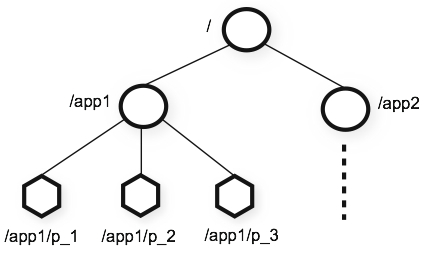
\includegraphics[width=0.4\textwidth]{software/zknamespace.jpg}
    \caption{A sample namespace}
    \label{fig:zk_namespace}
\end{figure}

These znodes can have different flags set which control their behavior. These are persistent, ephemeral and sequential. Persistent is self explanatory. When this flag is set during a put operation, the data will remain in ZooKeeper even though the client disconnects. Ephemeral is the opposite. Data placed in ZooKeeper with this flag will be deleted when the client loses its session. If sequential is set to be true then each child of the znode will have a monotonic increasing sequence number appended to its path. This number is relative to the parent znode, so children znodes can have equal or different names. Ephemeral and sequential are powerful features which enable us to utilize ZooKeeper for leader election, coordination as well as locks. 

\subsection{ZooKeeper Guarantees}
ZooKeeper provides two basic ordering guarantees:

\begin{itemize}
	\item Asynchronous linearizable writes
 	\item FIFO client order
\end{itemize}

Since we have asynchronous writes a client can have several outstanding operations, but ZooKeeper guarantees that they will be executed in FIFO order. ZooKeeper also provides clients with the option to listen for changes on a znode. ZooKeeper guarantees that a client will receive a changeEvent before see the new state of the system following the change. 

\subsection{Watches}
As mentioned above, a client can request a watch on a znode in ZooKeeper. This watch will give the client a changeEvent the next time this znode changes. These changes includes changes in number of children, change in data of znode or that the znode has been deleted. These watches can also be put on non existing znodes which gives the client an event when the znode is registered in ZooKeeper. It is however important to note that a watch will only trigger once, and it is not possible to request infinite watches. So it is up to each individual client to request a new watch after receiving an event.

Because of ZooKeepers linearizable guarantees a read following one of these watchEvents will always return the new state of the system. In the event of several changes in quick succession it is possible for a client to not be notified of each individual change. It will however always be able to determine the final state of the system after all the changes.

\subsection{Implementation}

As mentioned ZooKeeper can be used for more than just storing configuration data. In this section we will explain some different ways to use ZooKeeper with short psudo code examples. 

\subsubsection{Group membership}
ZooKeeper can be used to keep track of group membership. To do this we create a znode for the group at a given path. Now members can register their membership by creating a child znode with the ephemeral flag set. As long as they have a session with ZooKeeper they will be listed as a member of the group. When a member registers as a child they also put a watch on the parent node. If there is a change in membership, for example a node is added, then all nodes set to watch for changes will receive an event. Because of ZooKeepers FIFO ordering guarantees we will never have the case that a node is added some existing node is not notified. 

\subsubsection{Leader election}
Leader election is something that frequently needs to be addressed in a distributed system. In our own Headmaster client we used ZooKeeper to handle this issue. 

To elect a leader we utilize the sequential and ephemeral flags of a znode. We have a znode called leaders in ZooKeeper where potential leaders can register themselves. This znode has the sequential flag set so we get a total order on the potential leaders. We also force each potential leader to use the ephemeral flag when registering. This ensures that when a client disconnects it is removed from the leader znode.By default the znode with the lowest sequence number will be the one that is the leader.

If a potential leader does not win the election (I.E: There is another contender with a lower sequence number) it puts a watch on the winner and waits for changes. If eventually the leader disconnects then there will once again be elected a new leader based on sequence number.

Any client wanting to get a hold of its leader can simply ask ZooKeeper for all the children of the leader znode, and then determine which one is the leader based on sequence numbers. Now the client can put a watch on this leader znode and be notified whenever there is a change in leadership. If said event is received the client simply ask ZooKeeper again for the children and repeat the process.

\subsubsection{Locks}
Another typical use case for ZooKeeper is handling locks. The way we implement locks is by having a reserved path for a znode called lock in ZooKeeper. To control the lock a client must be the one to create this znode with the ephemeral flag set. We use ephemeral to prevent a client for keeping the lock forever in case of a disconnect. 

Any client wanting to use the resource related to the lock will try to create the lock znode. On success that client have access to the resource while in case of a failure the client will put a watch on the lock and wait for the existing znode to be deleted before trying to create it again.

It is also possible to separate locks into read and write locks. In ZooKeeper their only difference will be in the naming of the znode, but the client now can regard them as read or write locks. The case explained above is a typical write lock. In the case of a read lock, the client will be allowed access to the resource as long as there is no write locks before it. If there is a write lock ahead of the read the client will put a watch on said lock and wait until it is deleted. 






 

\clearpage

% implementation.tex

Our work and implementation happened mainly in 3 parts. Part 1 consists of integrating ZooKeeper support and mechanisms into a Voldemort server. Making Voldemort read configurations and storing data in ZooKeeper. Part 2 contains our work towards rebalancing by the help of ZooKeeper. In Part 3 we create the service Headmaster, which is a process to run along side of the Voldemort process. Headmaster listens to active nodes in the cluster, and can generate configuration for new nodes, add them to the cluster, and prepare the members for a rebalance to include the new node. Lastly we have included a part (\ref{sec:testing}) about how we validated our implementation while working.


\section{Part 1}
Integrating ZooKeeper into Voldemort and taking advantage of the coordination services ZooKeeper provides, proved rather difficult.
We chose to override and rewrite much of the current MetadataStore implementation to one that uses ZooKeeper as the backend storage engine instead of local files. 
Actual data is still of course stored locally, but configuration (meta data) now resides in the ZooKeeper cluster.
This abstraction works rather well for shared data files, but causes some issues with information that is stored for individual nodes. 
As such, we landed on a fixed path scheme, where certain configuration files are expected to reside on known locations, and will be presented later.

This change introduces the dependency of a running ZooKeeper cluster for normal operation of any node. While this is a liability and potential source for downtime in a highly available system, ZooKeeper is itself a highly available system and the 5 node setup is regarded as very stable and in heavy use at Yahoo\cite{need:citation}.
TODO: CITATION

Alternatively we could have made the coordination service optional, but we then considered it risky to allow updating config files live through ZooKeeper. In any case, the system will in general be able to operate through short ZooKeeper outages, as all meta and config data is cached locally, however changes will not propagate to the affected nodes as quickly.

\subsection{Configuration}
Configuration is stored in a VoldemortConfig object. Normally this is created from settings stored in local files per node. At startup, the code looks for a properties file in a directory given by environment variable \texttt{VOLDEMORT\_HOME}. 

Now, if you specify a ZooKeeper connection URL as a command line parameter, the program looks for configuration in ZooKeeper.
We have given an example outline of the expected directory structure in Figure \ref{fig:configdirs}. This is for the three nodes \texttt{vold0.idi.ntnu.no}, \texttt{vold1.idi.ntnu.no} and \texttt{vold2.idi.ntnu.no}. You can see the expected path follows the pattern \texttt{/config/HOSTNAME/server.properties}. 

The startup code then reads the config file and tries to parse. If parsing fails, the server is set to fail to clearly signal something is wrong at startup, and needs immediate fixing. If the file is not found, the server registers a watch on the path in ZooKeeper. If there is a write to this file, ZooKeeper will let the server know and the config file can be re-read. 

One can argue whether to fail or listen when a config is not found, but we decided for the latter, to listen for changes, after implementing the management service. As we later will see, listening allows us to push new config files to a node by the help of our management daemon Headmaster. 

\begin{figure}[h]
\dirtree{%
.1 / \ldots{} \begin{minipage}[t]{8cm}(root directory)
			  \end{minipage}.
.2 config.
.3 nodes \ldots{} (individual node configs).
.4 vold0.idi.ntnu.no \ldots{} (hostname).
.5 server.properties.
.5 server.state.
.5 node.id.
.4 vold1.idi.ntnu.no.
.5 server.properties.
.5 server.state.
.5 node.id.
}
\caption{Individual node configs in the shared space.}
\label{fig:configdirs}
\end{figure}

Our modification inherits from the original VoldemortConfig object, so that the ZooKeeper capable version can be used in the same code, in the same manner. The modified code reads data from a fixed location in ZooKeeper, and sets the necessary settings and properties for the server to boot and join the cluster. The ZooKeeper connection URL is passed as a command line parameter.

The directory structure for the whole program can be viewed in its entirety in Figure \ref{fig:dirstruct}, and has been included for completeness.

\begin{figure}[h]
\dirtree{%
.1 / \ldots{} \begin{minipage}[t]{8cm}(The root can also be a chroot{.})
			  \end{minipage}.
.2 active .
.3 vold0.idi.ntnu.no \ldots{} (ephemeral).
.3 vold2.idi.ntnu.no \ldots{} (ephemeral).
.2 config \ldots{} (persistent) . 
.3 nodes (individual node configs).
.4 vold0.idi.ntnu.no.
.5 server.properties.
.5 server.state.
.5 node.id.
.4 vold1.idi.ntnu.no.
.5 server.properties.
.5 server.state.
.5 node.id.
.4 vold2.idi.ntnu.no.
.5 server.properties.
.5 server.state.
.5 node.id.
.3 cluster.xml.
.3 stores.xml.
.2 headmaster.
.3 headmaster\_0009 \ldots{} (ephemeral \& sequential).
.3 headmaster\_0011 \ldots{} (ephemeral \& sequential).
.3 headmaster\_0012 \ldots{} (ephemeral \& sequential) .
}
\caption{Directory structure in ZooKeeper. The nodes or directories are actually Znodes and can hold data.}
\label{fig:dirstruct}
\end{figure}

\subsection{MetadataStore}
The internal state for a node is written to a \texttt{Store} called \texttt{MetadataStore}. It consists of an in memory cache store, and a persistent one to disk. The different stores are implementations of an abstract data \texttt{Store}. As such, we wrote a \texttt{Store} using ZooKeeper as the backend, and used this for persistent storage.

At startup we read the global configuration, the cluster and stores settings, from the Store. The Store fetches the requested files from ZooKeeper, and leaves a watch on the nodes. Because a store \emph{only} \emph{stores} data, the Store itself can not take advantage of the event deliveries from ZooKeeper: The Store keeps no application logic, and can be thought of as a hash map.

To notify and update the internal state of the node on events, we found it necessary to receive events in the configuration management logic, written in the \texttt{MetadataStore}.

When an event from the ZooKeeper client is delivered to the \texttt{MetadataStore}, we first sort it by type.
If it is a management event, like a disconnect event, we temporarily disable the ZooKeeper backend and serve data from the cache until it is reconnected. In our testing, such disconnects (session expiry) happened about once every hour, but the reconnect was usually done in less than two seconds. This instability may be due to our ZooKeeper cluster consisting of a single node and being on a different network.

After a session expiry, we receive a reconnected event when the ZooKeeper client reestablishes a connection. At this point, all set watches are lost, and all events during the connection loss will have been lost. We must therefore reset all watches and check the global configuration data on reconnect. 

\section{Handling the ZooKeeper connection}
Our handling of the ZooKeeper client and connection went through many stages and changes as we got a better understanding of its features.

Our currently preferred design can be viewed in \texttt{ActiveNodeZKListener}.
The ActiveNodeZKListener class wraps a ZooKeeper client connection, providing event delivery to the interface \texttt{ZKDataListener}. 
This approach removes a lot of the noise generated by the client, and delivers clear events that are simpler and clearer to handle and reason with when coding application logic.

We provide the following listener events:
\begin{description}

	\item[dataChanged(path):] 
		This method is called when data has been written to the watched Znode on \texttt{path}.
	\item[nodeDeleted(path):] 
		A call to the listener to let it know the Znode on \texttt{path} has been deleted.
	\item[reconnected():] 
		The connection handler provides a simple call \texttt{reconnected()} when a connection is reestablished after session expiry. When this call happens, we know it is safe to do sanity checking of our state and register watches again.
	\item[childrenList(path):]
		This one is a little bit special. This method is called whenever a Znode's children list is changed. Recall that Znodes are like nodes in a tree, and can have many children. This method call indicates new or removed children for the node on \texttt{path}.

\end{description}

We also include the possibility for receiving the raw events from the ZooKeeper client in the interface:

\begin{description}
	\item[process(event):]
		\texttt{Event} is the raw WatchedEvent from the ZooKeeper client. Registering as a \texttt{Watcher} will forward every internal ZooKeeper event to the listener.

\end{description}




\section{Part 2}

\subsection{Initial configuration}


\subsection{Rebalance}
Another issue we bumped into is related to the architecture of Voldemort.
In a rebalance, the new config files are pushed (written) to each node separately using Voldemort admin data requests. This causes every node to execute a put of the new data on the MetadataStore.

As explained above, we use ZooKeeper for (persistently) sharing the global configuration files.
Also, we would like to be notified about changes to the config files using watches. So first you have N nodes in the cluster, executing N writes to the same file. Each file write potentially triggers N watches, causing a read and watch reset. Worst case we will end up with N writes and N*N watch triggers and reads, all in quick succession (less than a second).
We therefore decided to ignore such put requests in the ZooKeeper driven persistent Store, and only put the new data in the Metadata cache store, deferring the admin to use a ZooKeeper write operation to put the new config out, making the nodes do a re-read.


\subsection{Begrepsavklaring}
A \texttt{write} or \texttt{put} in the context of ZooKeeper is considered a ZooKeeper \texttt{setData} operation.

A ZooKeeper event, is an event triggered by a watch set in ZooKeeper, giving push information about a change in ZooKeeper about a znode being watched.

In the context of ZooKeeper, the word file might be used for a znode. File used in the context of a local filesystem is a local file.

\section{Part 4}
\label{sec:testing}
TODO: Tests and unit tests?
When working on large projects, a lot of code lines are involved. To prevent breaking functionality underway, and to help verify correct (desired) behavior while working, we decided to write unit tests. 
Because of the complex series of events that need to happen while running the program to execute your desired code, it is much easier and more efficient to test and verify your code programmatically in a test environment. The design and verification of our Headmaster program greatly benefited from this approach. The event chain to test the code can be fairly complex, even though the application logic is fairly straight forward.

To create a test environment, we used JUnit and the Mockito project to mimic the behavior we need for validation.
Mockito is a testing framework for Java. It allows to create ``mock'' objects that can be used to trigger and verify program behavior in a predictable and controlled manner. The ``fake'', but controllable objects are very useful for eliminating outer dependencies, and instead having them behave in a completely predictable and controlled way.

Listing \ref{lst:mockito} shows a short example of how Mockito and JUnit is used to write short, simple yet powerful functional tests that verify behavior. It is also worth noting that the resulting test code is quite readable by a programmer.

\begin{lstlisting}[style=customjava,label=lst:mockito,caption={Test code utilizing Mockito. Think of the \texttt{@Mock} class as a subclass with all methods overrided \texttt{return null;}.}]
$$@Mock
ActiveNodeZKListener activeNodeZKListener;

Headmaster headmaster;

public void whenDataChangedTestIfWatchIsReset() {
    String path = "/config/cluster.xml";

    when(activeNodeZKListener.getStringFromZooKeeper(
    	path, true)).thenReturn(EXAMPLE_CLUSTER);

    headmaster.setZKListener(activeNodeZKListener);

    headmaster.dataChanged(path);

    /** 
     * verify method is called with params path, and watch flag set to true.
     */
    verify(activeNodeZKListener, times(1)).getStringFromZooKeeper(path, true);
}

\end{lstlisting}

Here we are verifying that upon receiving a notification that a znode has changed, the Znode (path) is fetched with a new watch set.
All without actually providing a working third party object (ActiveNodeZKListener) to the test, the object is entirely faked with the static \texttt{when} and \texttt{thenReturn} methods. After setting the dependency class up with the desired behavior, it is injected into the class we are testing, then verify that the desired method is called once and only once (\texttt{times(1)}). Similarly it is easy to see how you can verify two calls (\texttt{times(2)}). For zero calls, it is recommended to use the more readable method \texttt{never}.

\clearpage

\clearpage

\section{Hardware}
\label{sec:hardware}

\subsection{Mac Mini}
We server running voldemort is a a Mac Mini Mid 2010 model. It has a Intel Core Duo 2.4 GHz processor, 8 GBs of RAM and solid state storage. We run the latest OS X 10.9.1

\begin{figure}[h]
    \centering
    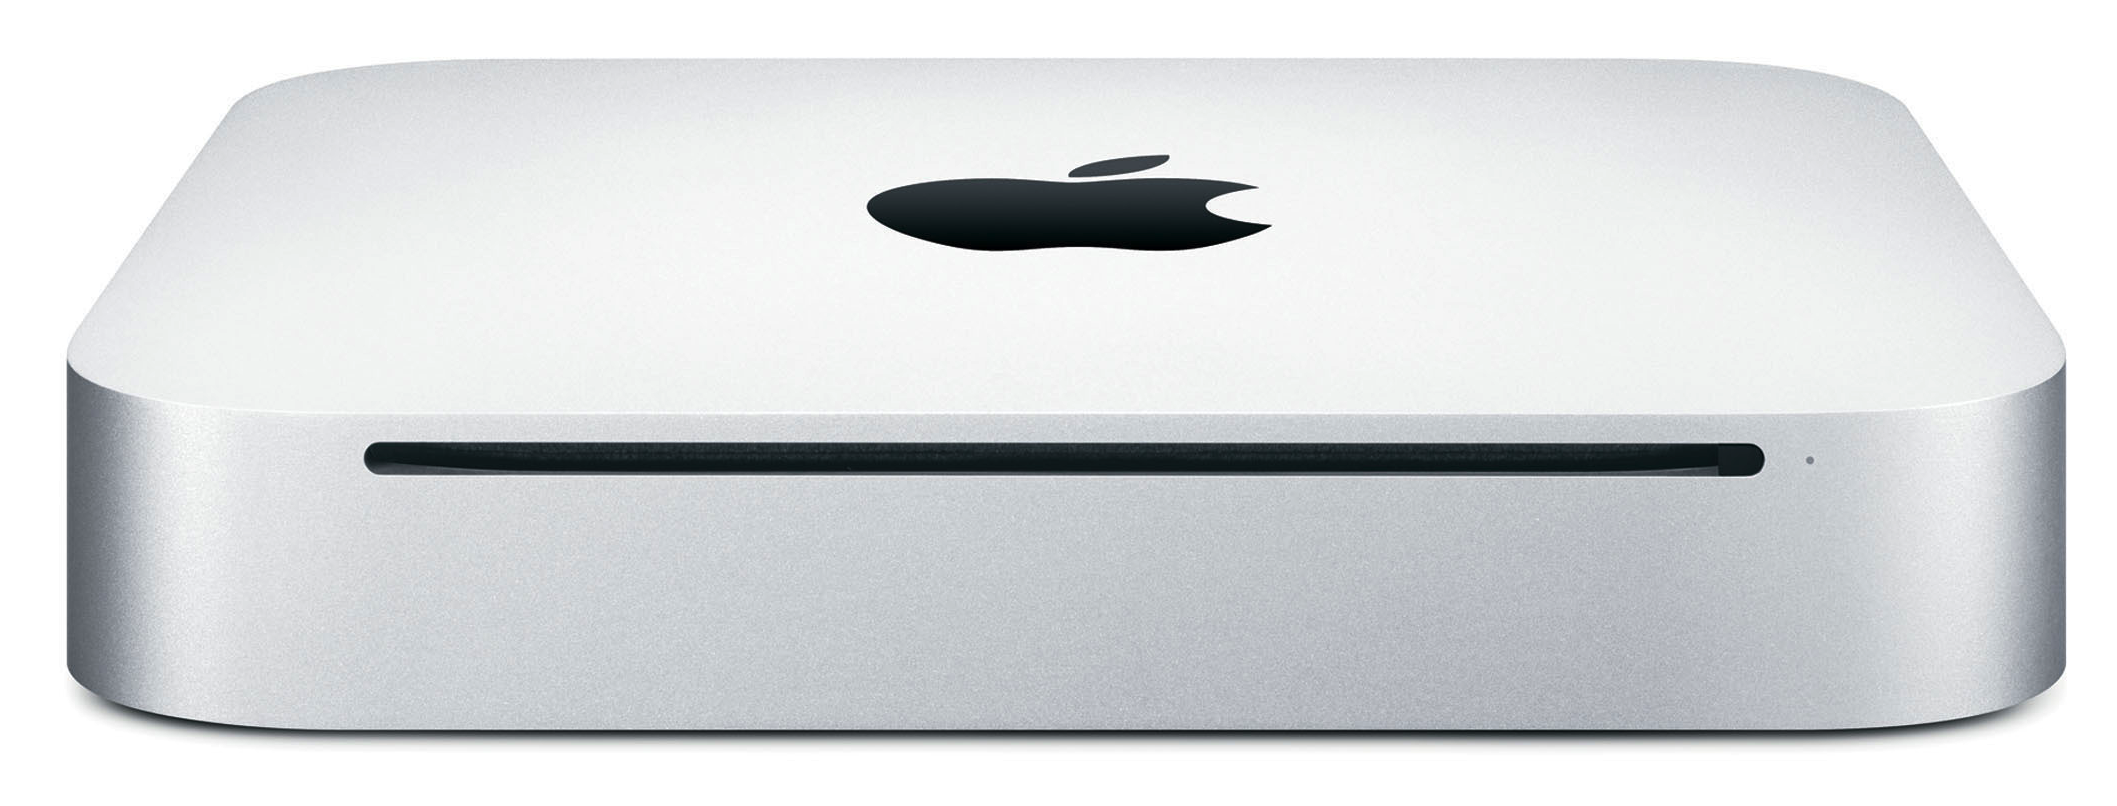
\includegraphics[width=0.8\textwidth]{hardware/mac-mini-06-2010}
    \caption{Mac Mini 2010}
    \label{fig:macmini_hw}
\end{figure}


\clearpage

\bibliographystyle{plain}
\bibliography{references}

\end{document}
